\documentclass[t,aspectratio=169, 8pt]{beamer}
\usetheme{baurg}
\usepackage{rg-code-beamer}

\usepackage[english]{babel}
\usepackage{subcaption}
% Maths and Physics
\usepackage{amsmath}
\usepackage{amsthm}
\usepackage{amssymb}
\usepackage{physics}
\usepackage{tabularx}
\usepackage{braket}
\usepackage{bm}
\usepackage{array,multirow,graphicx}


\def\*#1{\bm{#1}}

% For figures
\usepackage{tikz}
\usetikzlibrary{decorations.pathmorphing}
\usetikzlibrary{shapes}
\usetikzlibrary{matrix,shapes.geometric}
\usetikzlibrary{positioning,fit,calc} 
\usepackage{svg}
\usepackage{subcaption}

\title{Solvatochromic Shifts in the Spectroscopy of Acetone}
\subtitle{\Large with LAMMPS and VOTCA}
\author{August 13, 2021}
\department{LAMMPS Virtual Workshop 2021}

\begin{document}

\begin{titleframe}[variant=1,bgimage=background.png]
\end{titleframe}

\begin{chapterframe}
  \frametitle{Overview}
  \begin{itemize}
    \item How to follow along
    \item The QM/MM Approach
    \item Doing QM/MM with LAMMPS AND VOTCA
  \end{itemize}
\end{chapterframe}


%%%%%%%%%%%%%%%%%%%%%%%%%%%%%%%%%%%%%%%%%%%%%%%%%%%%%%%%%%%%%%%%%%%%%%%%%%%%%%%
% SETUP OF THE TUTORIAL
%%%%%%%%%%%%%%%%%%%%%%%%%%%%%%%%%%%%%%%%%%%%%%%%%%%%%%%%%%%%%%%%%%%%%%%%%%%%%%%%

\begin{frame}[fragile]
  \frametitle{How to follow along}
  You can follow along with this tutorial on you own pc, assuming you can run docker. To set it up on a Ubuntu machine, install docker,
  \begin{minted}{bash}
sudo apt install docker.io
  \end{minted}
  and pull the votca image.
  \begin{minted}{bash}
sudo docker pull votca/votca
  \end{minted}
Next we start docker and load the environment variables of VOTCA
  \begin{minted}{bash}
sudo docker run -it votca/votca /bin/bash
source VOTCARC.bash
  \end{minted}
  To find all the necessary input files \mintinline{bash}{cd} to 
\begin{minted}{bash}
cd xtp-tutorials/LAMMPS_workshop
\end{minted}
Now you are all set to follow along. 

\end{frame}


%%%%%%%%%%%%%%%%%%%%%%%%%%%%%%%%%%%%%%%%%%%%%%%%%%%%%%%%%%%%%%%%%%%%%%%%%%%%%%%
% THE QMMM APPROACH
%%%%%%%%%%%%%%%%%%%%%%%%%%%%%%%%%%%%%%%%%%%%%%%%%%%%%%%%%%%%%%%%%%%%%%%%%%%%%%%%
\begin{frame}
  \frametitle{The QM/MM Approach}
  \centering
  \includegraphics[height=0.65\textheight]{images/siteenergies}
\end{frame}

\begin{frame}
  \frametitle{The QM/MM Approach: A combination of 4 models}
  \begin{columns}[t]
    \begin{column}{0.44\textwidth}
        \begin{itemize}
          \item Molecular Dynamics:
          \begin{itemize}
            \item Used to obtain a snap shot of the topology of the molecular system
            \item \textbf{Tool:} LAMMPS (or GROMACS)
            \item \textbf{Representation:} Geometry + Forcefield
          \end{itemize}
          \item Quantum Mechanical:
          \begin{itemize}
            \item Used to compute the excited states of a molecule and generate input files.
            \item \textbf{Tool:} VOTCA (excited states) + ORCA (input files) 
            \item \textbf{Representation:} Optimized geometry
          \end{itemize}
        \end{itemize}
    \end{column}
    \begin{column}{0.44\textwidth}
      \begin{itemize}
        \item Electrostatics:
        \begin{itemize}
          \item The electrostatics are computed based on a multipole expansion (in this tutorial just partial charges).
          \item \textbf{Tool:} VOTCA (and ORCA)
          \item \textbf{Representation:} Distributed multipoles
        \end{itemize}
        \item Polarization:
        \begin{itemize}
          \item We use the applequist model with Thole damping, i.e. polarizable dipoles.
          \item \textbf{Tool:} VOTCA (and ORCA)
          \item \textbf{Representation:} Distributed polarizabilities
        \end{itemize}
      \end{itemize}
  \end{column}
\end{columns}
\vspace{0.5cm}
To do a QM/MM calculation we need to setup the representations for each model and generate all the necessary input files.
\end{frame}


%%%%%%%%%%%%%%%%%%%%%%%%%%%%%%%%%%%%%%%%%%%%%%%%%%%%%%%%%%%%%%%%%%%%%%%%%%%%%%%%
% QMMM WITH VOTCA
%%%%%%%%%%%%%%%%%%%%%%%%%%%%%%%%%%%%%%%%%%%%%%%%%%%%%%%%%%%%%%%%%%%%%%%%%%%%%%%%
\begin{chapterframe}
  \frametitle{Performing QM/MM with VOTCA and LAMMPS}
  The process of performing a QM/MM calculation consists of three general steps.
  \begin{enumerate}
    \item Create representations and input files
    \item The mapping procedure (combining the representations from the 4 models)
    \item Running the QM/MM calculation
  \end{enumerate}
\end{chapterframe}

\begin{frame}[fragile]
  \frametitle{The System and Generating Input Files}
  \begin{columns}[b]
    \begin{column}{0.58\textwidth}
  \textbf{The MD trajectory of Acetone in Water}\\
  The MD trajectory can be obtained by running a normal LAMMPS simulation of your system. For this tutorial we have already performed the MD simulation for you. The relevant data can be found in the \mintinline{bash}{system.data} and \mintinline{bash}{traj1.dump} files.
  \vspace{0.3cm}\\
  \textbf{Optimized geometries}\\
  Optimized geometries can be obtained from many QM packages including VOTCA. For this tutorial we have already computed them with ORCA. The ORCA results and the input files that generated them can be found in the \mintinline{bash}{DFT_ORCA} folder. 
  \vspace{0.3cm}\\
  \textbf{Multipoles and Polarization}\\
  The multipoles and polarization can also be computed with ORCA and that is what we did for this tutorial.The ORCA output files, however, need to be converted to a VOTCA readable format called mps files. 
\end{column}
\begin{column}{0.4\textwidth}
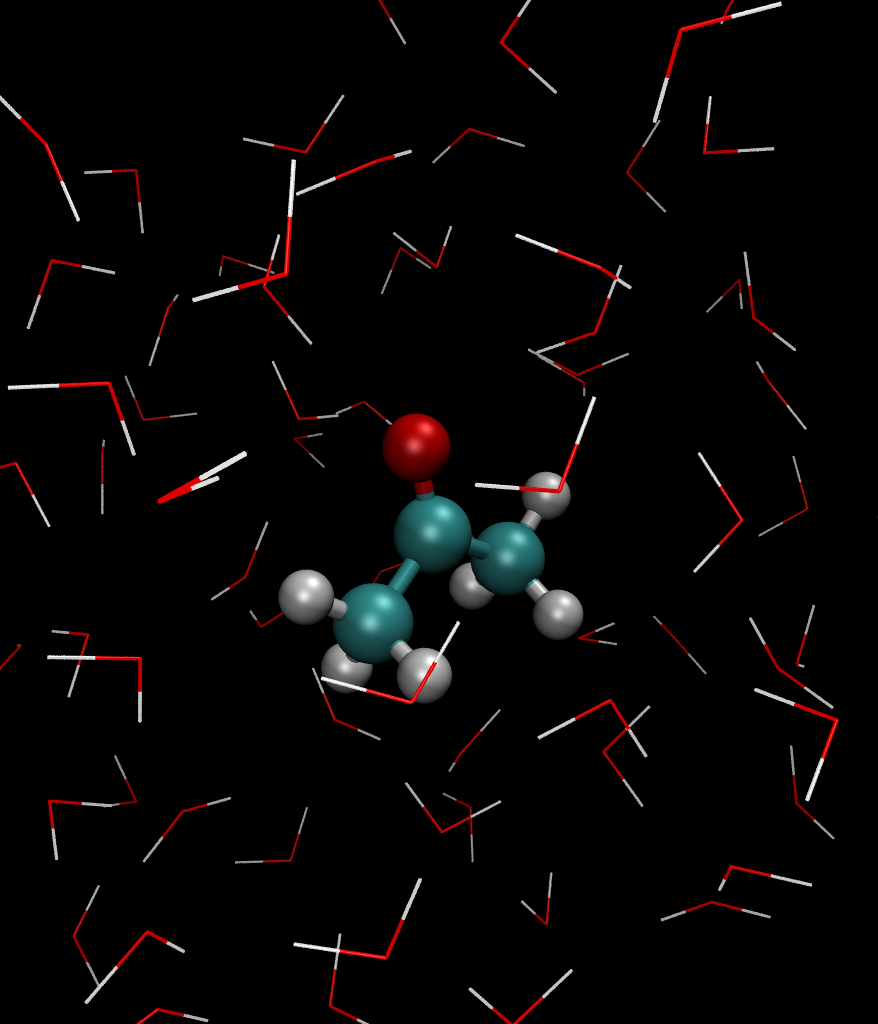
\includegraphics[width=0.95\textwidth]{system}
\end{column}
\end{columns}
\end{frame}

\begin{frame}[fragile]
  \frametitle{Generating the Multipole and Polarizability files}
  For the multipoles and polarization VOTCA uses mps files. There is a special tool in VOTCA that converts ORCA log files with CHELPG charges to an mps file.  
  \begin{minted}{bash}
xtp_tools -e log2mps -o OPTIONS/log2mps_water.xml
  \end{minted}
  We see here the typical way of calling a VOTCA program
  \begin{minted}{bash}
xtp_<executableType> -e <calculationType> -o <optionsFile>.xml
  \end{minted}
  The option file
  \begin{minted}{xml}
<options>
    <log2mps>
        <dftpackage>orca</dftpackage>
        <input>DFT_ORCA/water/chelpg.log</input>
        <output>MP_FILES/water_n.mps</output>
    </log2mps>
</options>
  \end{minted}
\end{frame}

\begin{frame}[fragile]
  \frametitle{How to find out which options are available?}
  \begin{enumerate}
    \item Look at the description of a program with the describe flag \mintinline{bash}{-d}\\
      \begin{minted}{bash}
xtp_tools -d log2mps
    \end{minted}
    \item Print (\mintinline{bash}{-p}) an example options file with \textbf{all} available options to an output file (\mintinline{bash}{-o})
    \begin{minted}{bash}
xtp_tools -p log2mps -o optionsLog2mps.xml
    \end{minted}
  \end{enumerate}
\end{frame}


\begin{frame}[fragile]
  \frametitle{The result of \textit{log2mps}}  
  The generated MPS file.
  \begin{minted}{text}
! GENERATED BY VOTCA::XTP::::LOG2MPS 
! N=3 Q[e]=+0.0000000
Units angstrom
  O +0.0000000 +0.0000000 -0.0043320 Rank 0
    -0.7585550
    P +0.8370000
  H +0.7614610 +0.0000000 +0.5795250 Rank 0
    +0.3787500
    P +0.4960000
  H -0.7614610 +0.0000000 +0.5795250 Rank 0
    +0.3798050
    P +0.4960000
  \end{minted}
  But the polarizations are still wrong.
\end{frame}

\begin{frame}[fragile]
  \frametitle{Fitting Polarizabilities}  
  To obtain the atomic polarizabilities we fit them such that they represent the
  molecular polarizabillity as close as possible. The molecular polarizabilities
  are calculated with ORCA for this tutorial. VOTCA has a tool specifically for
  this fitting procedure.
  \begin{minted}{bash}
xtp_tools -e molpol -o OPTIONS/molpol_water.xml
  \end{minted}
  The options file
  \begin{minted}{xml}
<options>
  <molpol>
    <input>MP_FILES/water_n.mps</input>
    <output>MP_FILES/water_n_pol.mps</output>
    <mode>qmpackage</mode>
    <qmpackage>orca</qmpackage>
    <logfile>DFT_ORCA/water/chelpg.log</logfile>
  </molpol>
</options>
  \end{minted}
  Check the output file.
\end{frame}


%%%%%%%%%%%%%%%%%%%%%%%%%%%%%%%%%%%%%%%%%%%%%%%%%%%%%%%%%%%%%%%%%%%%%%%%%%%%%%%%
% MAPPING 
%%%%%%%%%%%%%%%%%%%%%%%%%%%%%%%%%%%%%%%%%%%%%%%%%%%%%%%%%%%%%%%%%%%%%%%%%%%%%%%%


%%%%%%%%%%%%%%%%%%%%%%%%%%%%%%%%%%%%%%%%%%%%%%%%%%%%%%%%%%%%%%%%%%%%%%%%%%%%%%%%
% QUESTIONS
%%%%%%%%%%%%%%%%%%%%%%%%%%%%%%%%%%%%%%%%%%%%%%%%%%%%%%%%%%%%%%%%%%%%%%%%%%%%%%%%
\begin{chapterframe}
  \frametitle{Results}
  \vspace{0.5cm}
  \begin{center}
    {\fontsize{60}{64} \selectfont \bfseries{?}}
  \end{center}
\end{chapterframe}


\end{document}